\chapter{System Architecture and Methodology}
\label{ch:architecture}

\section{The Decision}
\label{sec:decision}

We implement a \textbf{Lambda architecture}: an immutable master dataset
written by a dedicated archiver, a \emph{speed layer} computing
approximate live views, and a \emph{batch layer} recomputing exact views
from the complete archive. Figure~\ref{fig:architecture} shows the
resulting system.

\begin{figure}[htbp]
\centering
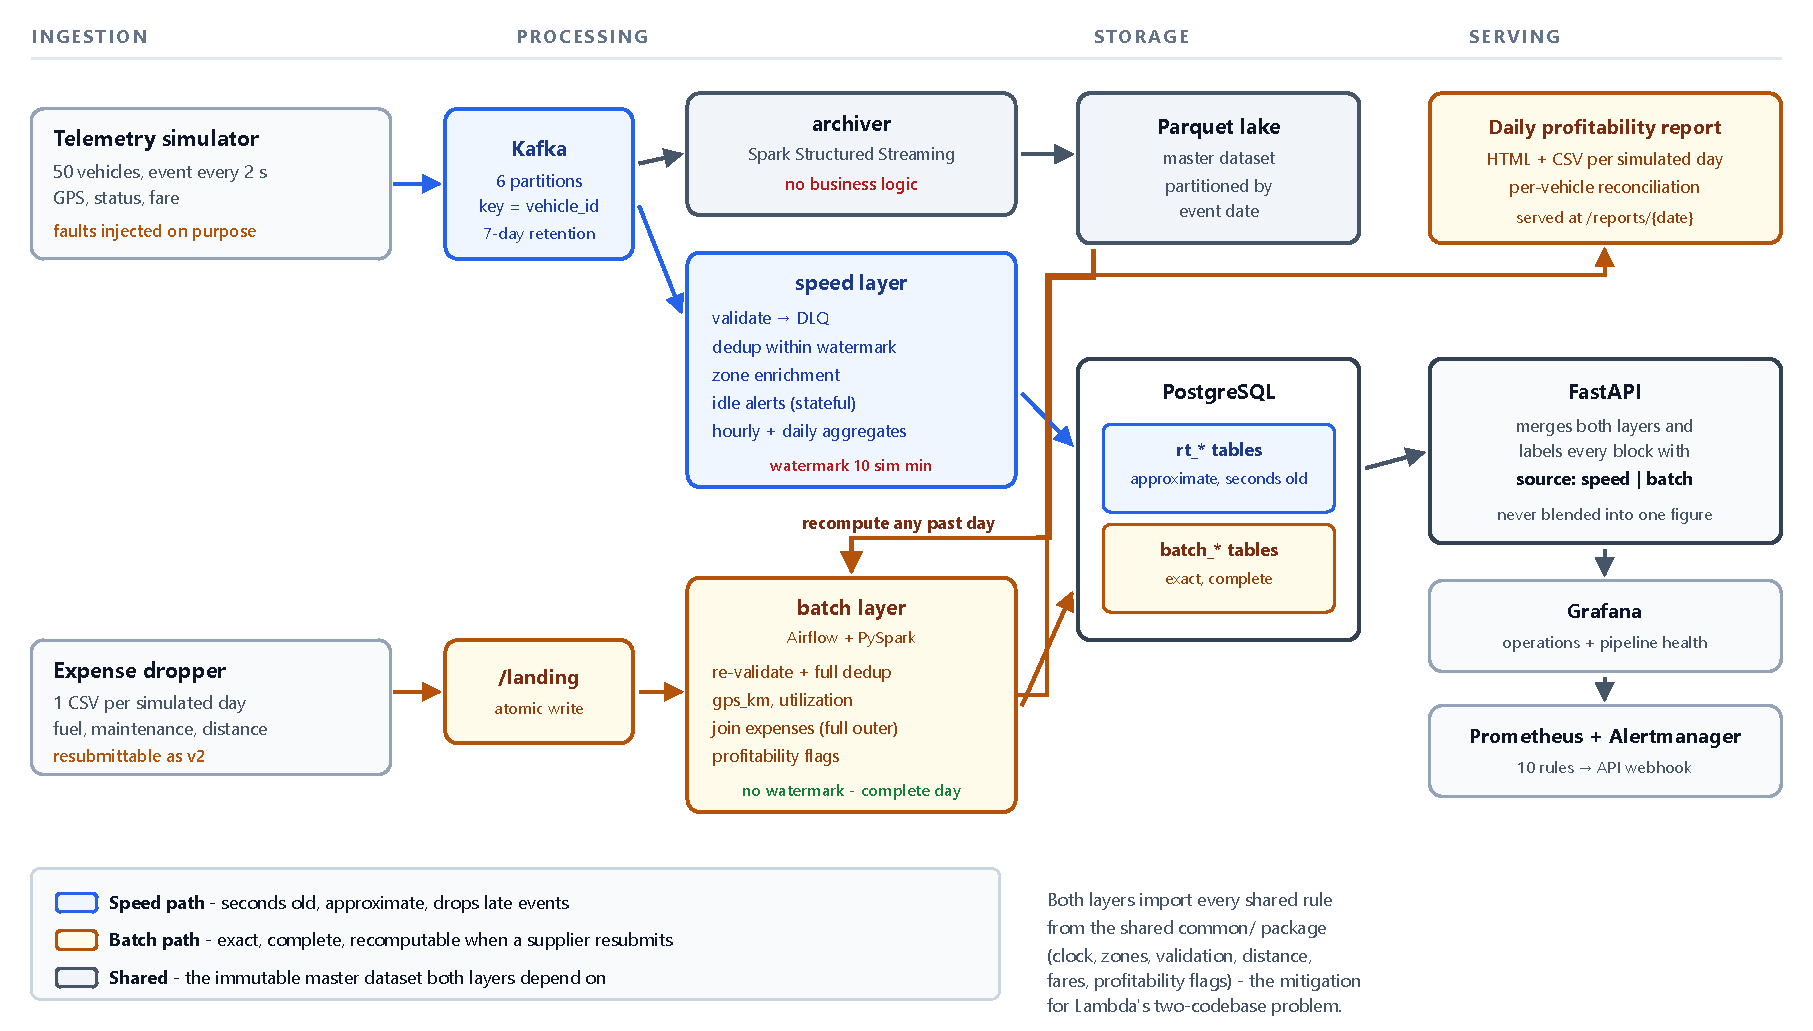
\includegraphics[width=\textwidth]{figures/fig1-architecture.pdf}
\caption[System architecture]{System architecture. The blue path is the
speed layer (seconds old, approximate); the amber path is the batch layer
(exact, complete, recomputable). Both depend on the same immutable master
dataset, and both import every shared business rule from
\code{common/}.}
\label{fig:architecture}
\end{figure}

The decision follows from Table~\ref{tab:two-questions} rather than from
a preference for a named architecture. Two consumers need different
guarantees from the same facts; a single processing model must either
under-serve one or lie to the other.

\section{Why Kappa Was Rejected}
\label{sec:kappa-rejected}

Kappa proposes a single streaming layer, with recomputation achieved by
replaying the event log~\cite{kreps2014questioning}. It is the more
fashionable choice, it is genuinely simpler to operate, and its critique
of Lambda's duplicated logic is correct. It therefore deserves a specific
rejection rather than a dismissal.

\textbf{The decisive argument is recomputation cost.} Our requirement is
not merely to reprocess data --- it is to \emph{restate a past day's
financial figures} when a partner sends corrected costs. Under Kappa that
implies three things:

\begin{enumerate}
  \item \textbf{Retention must cover any day we might be asked to
        restate.} A partner correcting last month's file forces months of
        Kafka retention purely to enable periodic recomputation. Our
        actual retention is \textbf{7 days}, and it covers only
        speed-layer recovery and archiver catch-up.
  \item \textbf{Replay is not selective.} Recomputing one day means
        re-reading the log from at least that day's start. A Parquet lake
        partitioned by \code{sim\_date} lets the batch job read exactly
        the one partition it needs; the measured
        \code{compute\_vehicle\_day} task takes \textbf{9.4 seconds} for
        a full simulated day.
  \item \textbf{The correction is not in the stream at all.} The expense
        file arrives on a \emph{different channel} --- a CSV drop --- once
        per day, long after the telemetry it relates to. There is no
        event log to replay that would incorporate it. Kappa's
        recomputation story simply does not address the actual source of
        restatement.
\end{enumerate}

The third point is the structural one, and it is what
Section~\ref{sec:lit-gap} identified as the condition under which the
literature's decision rule selects Lambda. A Kappa purist could of course
publish the expense file onto a topic and treat it as a second stream.
That is a real option, and we considered it; it relocates the problem
rather than solving it, because restating January from a corrected file
received in March still requires the January \emph{telemetry} to be
replayable, which is the retention cost of point~1 in a different guise.

A \textbf{batch-only architecture} was also considered and rejected for
the obvious reason: it cannot answer ``which vehicles are idle right
now''. The brief requires a live utilisation endpoint and threshold
alerting on idleness, neither of which survives a nightly cadence.

\section{What Lambda Costs, and Our Mitigation}
\label{sec:lambda-cost}

The standard criticism of Lambda is \textbf{two codebases that
drift}~\cite{kreps2014questioning}: the same business rule gets written
once for streaming and once for batch, and the two copies diverge until
the layers silently disagree. We accept the criticism as valid and
mitigate it structurally rather than by promising discipline.

A \code{common/} package holds every rule both layers need --- the
simulated clock, zone mapping, event validation, haversine distance, fare
maths and all seven profitability flags --- and is imported by the
simulators, the speed layer, the batch layer \emph{and} the serving API.
A business rule defined twice is treated as a defect.

Two places duplicate deliberately, both for performance, because a Python
UDF executing per row over every event is the most expensive thing this
pipeline could do. Table~\ref{tab:duplications} lists them with the test
that pins each pair together.

\begin{table}[htbp]
\centering
\caption{The two deliberate duplications, and the tests that make them
defensible. Each test feeds identical inputs through both
implementations and asserts identical outputs.}
\label{tab:duplications}
\begin{tabularx}{\textwidth}{@{}lllX@{}}
\toprule
\textbf{Logic} & \textbf{Python} & \textbf{Spark} & \textbf{Test}\\
\midrule
Event validation & \code{validate\_event()} &
  \code{spark\_validation\_expr()} &
  \code{test\_spark\_validation\_matches\_the\_python\_rules}\\
Haversine distance & \code{geo.haversine\_km()} & inline Spark SQL &
  \code{test\_gps\_km\_matches\_the\_python\_haversine}\\
\bottomrule
\end{tabularx}
\end{table}

The duplication is a considered trade-off that is only defensible
\emph{because} those tests exist. Without them we would have precisely
the failure mode Kreps describes.

\section{Technology Stack}
\label{sec:tech-stack}

Table~\ref{tab:stack} gives each choice with the alternative it beat.
Justifications are tied to this use case's constraints, not to general
popularity. Every image tag and Python package is pinned; there is no
\code{latest} anywhere in the project.

\begin{table}[htbp]
\centering
\caption{Technology selection, with the rejected alternative for each
layer.}
\label{tab:stack}
\begin{tabularx}{\textwidth}{@{}llX@{}}
\toprule
\textbf{Layer} & \textbf{Choice} & \textbf{Why this, and not the
alternative}\\
\midrule
Ingestion & Kafka 3.8 (KRaft) &
  Partitioned ordering is a \emph{correctness} requirement here, not a
  throughput one (Section~\ref{sec:impl-partitioning}). KRaft removes
  the ZooKeeper dependency entirely, which halves the moving parts on a
  16\,GB laptop.\\
\addlinespace
Speed layer & Spark Structured Streaming 3.5.3 &
  Event-time windowing, watermarks and
  \code{applyInPandasWithState} in one engine~\cite{spark_ss_guide}.
  Flink is arguably the stronger stream processor in
  isolation~\cite{carbone2015flink}, but using \emph{one} engine for
  both layers is precisely what makes \code{common/} shareable, and the
  shared package is our answer to Lambda's central weakness.\\
\addlinespace
Master dataset & Parquet on a volume &
  Columnar, partitioned by event date, read
  selectively~\cite{parquet_docs}. MinIO was the intended object store
  but its community images are no longer published; every path is built
  from \code{LAKE\_ROOT}, so an \code{s3a://} bucket is a one-variable
  substitution.\\
\addlinespace
Batch & Airflow 2.10 + PySpark local mode &
  Airflow gives retries, dependency ordering and per-task
  observability~\cite{airflow_docs}. Local mode because one simulated
  day is roughly 12k events, which a single JVM processes in 9 seconds;
  client-mode submission would add driver/executor routing problems for
  no measurable gain.\\
\addlinespace
Serving store & PostgreSQL 16 &
  Both layers' views live side by side in one queryable
  store~\cite{postgres_docs}. Upserts on natural keys give idempotent
  sinks (Section~\ref{sec:impl-sinks}). Cassandra would suit the
  write-heavy \code{rt\_*} tables but not the analytical scans over
  \code{batch\_vehicle\_daily}, and running both was not justified at
  this volume.\\
\addlinespace
API & FastAPI &
  Pydantic response models make the \code{source: speed|batch} labelling
  part of the \emph{schema} rather than a
  convention~\cite{fastapi_docs}; the generated OpenAPI page doubles as
  the demo surface.\\
\addlinespace
Observability & Prometheus, Alertmanager, Grafana &
  Pull-based scraping suits long-lived
  services~\cite{prometheus_docs,grafana_docs};
  Section~\ref{sec:impl-observability} explains how short-lived Airflow
  tasks are handled without a Pushgateway.\\
\bottomrule
\end{tabularx}
\end{table}

\section{The Simulated Clock}
\label{sec:simclock}

Everything in this project happens on a compressed timeline:
\textbf{one real second is one simulated minute} (\code{COMPRESSION=60}).
A simulated hour therefore takes one real minute and a simulated day
takes 24 real minutes, which is what makes a genuinely \emph{daily}
reconciliation demonstrable inside a lab session.

The clock is derived from a persisted start instant rather than
maintained as a counter, so every service computes the same
\code{sim\_time} from wall-clock elapsed time without coordinating, and a
restarted container resumes on the same timeline instead of rewinding.
Simulated day~1 begins at 06:00 and is therefore partial.

This is the project's largest single simplification and it has a
consequence we report rather than hide: because simulated time is derived
from wall-clock time, \textbf{the pipeline being down does not pause the
world}. Section~\ref{sec:limitations} returns to this.

\section{The Data Contract}
\label{sec:contract}

Three fields were added to the telemetry schema given in the brief, each
for a specific architectural reason.

\begin{description}
  \item[\code{event\_id} (UUID)] Deduplication needs a stable identity.
        A duplicate is by construction \emph{valid}, so nothing in
        validation can catch it.
  \item[\code{event\_type} (\code{ping}/\code{trip\_start}/\code{trip\_end})]
        This one is structural. Without an explicit lifecycle marker,
        counting trips requires detecting a status \emph{transition} and
        then aggregating, which is a chained stateful operator ---
        and Structured Streaming forbids an aggregation after
        one~\cite{spark_ss_guide}. With the marker, ``trips completed''
        is a plain \code{count(WHERE event\_type='trip\_end')} that works
        identically in both layers.
  \item[\code{schema\_version} (int)] Allows a future v2 producer to
        coexist with v1 consumers.
\end{description}

One interpretation of an existing field matters downstream more than any
addition: \textbf{\code{fare} is cumulative within a trip and final only
on \code{trip\_end}}, and zero elsewhere. Revenue is therefore
\code{SUM(fare) WHERE event\_type='trip\_end'} in both layers. Summing
\code{fare} across all rows would multiply revenue by roughly the number
of pings per trip --- the single easiest way to get this pipeline's
headline number wrong --- so the rule carries a test in the simulator, the
speed layer and the batch layer.
